\documentclass[11pt, a4paper]{article}

\usepackage[utf8]{inputenc}
\usepackage[greek, english]{babel}
\usepackage{alphabeta}
\usepackage{libertine}
\usepackage{graphicx}
\usepackage{biblatex}[sorting=nty] % sort alphabetically
\usepackage[table]{xcolor}
\usepackage{mathptmx} % Times New Roman
\usepackage{makecell}
\usepackage{setspace}
\usepackage{geometry}
\usepackage{booktabs}

\pagenumbering{arabic}
\onehalfspacing % Set line spacing to 1.5
\graphicspath{ {./results/} }
\addbibresource{refs.bib}

\def\code#1{\texttt{#1}}

\title{\Huge Supplemental Material Part 1: Crawled Data Analysis\\
	\LARGE Practical Data Science: 2nd Project}

\author{\Large  Tsirmpas Dimitris }


\begin{document}
	
	\maketitle
	\begin{center}
		\large Athens University of Economics and Business \\
		\large MSc in Data Science
		
	\end{center}
	
	
	\section{Introduction}
	This report outlines results and conclusions drawn from the mechanical annotation of Greek and Greeklish YouTube comment data. The full report, detailing goals, data sources, methodology and implementation can be found at \url{https://github.com/dimits-exe/practical_data_science}.
	
	Our operational data have been collected by the top results of YouTube search for two categories: \textbf{Greek songs} and \textbf{Greek Gaming videos}. These categories represent two main demographics of the Greek online community: The older - middle-aged and the younger generations.
	
	
	\section{Language Identification Results}
	
	Below we present graphs resulting from the language identification analysis on the crawled YouTube dataset.
	
	\begin{itemize}
		\item Figure \ref{fig::lang_dis} illustrates the distribution of languages in our YouTube dataset. Unfortunately, our classifier did not perform as expected, showing a smaller preference for Greek and Greeklish than anticipated. This discrepancy may be attributed to insufficient training data or a lack of a representative sample from the crawled posts.
		
		\item Figure \ref{fig::emojis_dist} displays the number of emojis used in each comment, organized by comment language. Note that the plots are stacked, with each language on top of the previous one. To obtain the actual count for a specific language, deduct the count of emojis used in the previous language.
		
		\item Figure \ref{fig:length_dis} showcases the distribution of comment lengths for each language. An outlier is observed in an English comment that reached an unusually long 1500 characters. In general, Greek posts appear shorter, while English and Greeklish dominate the longer tail of the distribution.
		
		\item Figure \ref{fig::timeseries.png} features a time-series plot detailing the observed languages over dates. All languages exhibit a similar trend, indicating a probable absence of a statistically significant pattern. Most of the crawled videos, appearing in the YouTube search tab, are likely both relevant and popular. This explains why the majority of them are from the timeframe of 2020-2023.
	\end{itemize}
	
	
	
	\begin{figure}
		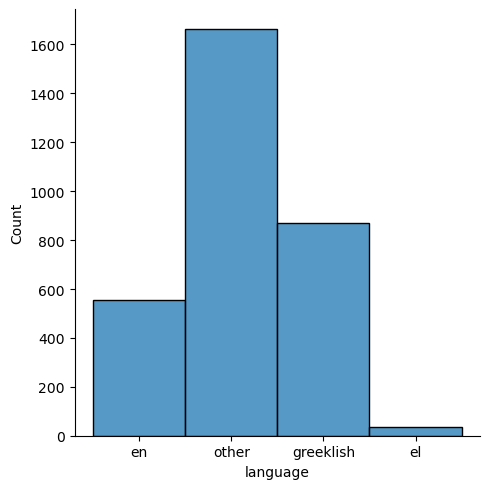
\includegraphics[width=10cm]{lang_dis.png}
		\centering
		\caption{Language distribution in the crawled dataset.}
		\label{fig::lang_dis}
	\end{figure}
	
	\begin{figure}
		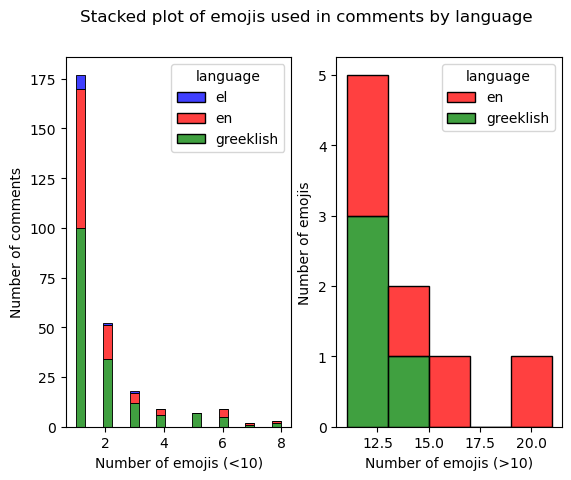
\includegraphics[width=10cm]{emojis_dis.png}
		\centering
		\caption{Stacked plot of emoji usage by language.}
		\label{fig::emojis_dist}
	\end{figure}
	
	\begin{figure}
		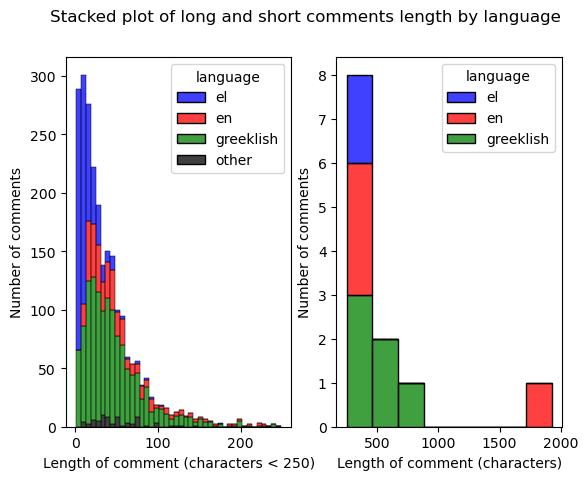
\includegraphics[width=10cm]{length_dis.png}
		\centering
		\caption{Length of comments by language, measured by characters.}
		\label{fig:length_dis}
	\end{figure}
	
	\begin{figure}
		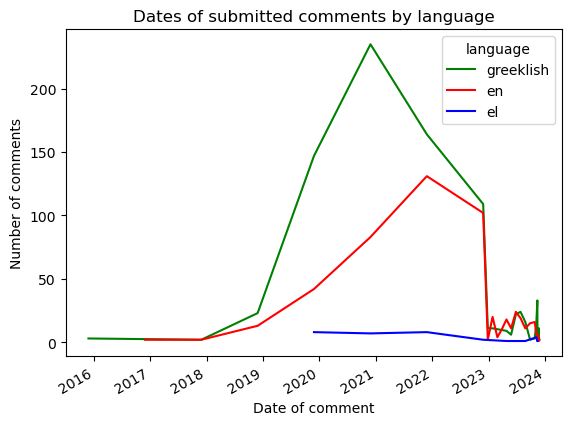
\includegraphics[width=10cm]{time_plot.png}
		\centering
		\caption{Number of comments by language for each day, running from 2017 to present.}
		\label{fig::timeseries.png}
	\end{figure}
	
	
	
	\section{Toxicity Classification Results}
	
	In this section we include the results of the toxicity analysis on the crawled data. The toxicity levels are defined as a scale from 1 to 5 where 1: Not Toxic, 	2: Maybe Toxic, 3: Almost Toxic,	4: Almost certainly Toxic, 5: Certainly Toxic.
	
	\begin{itemize}
		\item Table \ref{tab::toxic_lang} shows a breakdown of average comment toxicity per language. 
		
		\item Table \ref{tab::toxic_videos} shows the videos with the most toxic comments, sorted by descending toxicity.
		
		\item Table \ref{tab::toxic_uniform} shows the videos where the comment toxicity remained uniform across time.
		
		\item Table \ref{tab::toxic_increasing} shows the videos where the comment toxicity increased over time, as well as the average rate of increase. 
	\end{itemize}
	
	
	\begin{table}
\caption{Average toxicity by language.}
\label{tab::toxic_lang}
\begin{tabular}{|p{3.5cm}|p{1cm}|}
\toprule
language & toxicity \\
\midrule
el & 1.000 \\
en & 1.090 \\
greeklish & 1.011 \\
other & 1.000 \\
\bottomrule
\end{tabular}
\end{table}

	
	\begin{table}
\caption{The top 5 videos with the most toxic comments on average.}
\label{tab::toxic_videos}
\begin{tabular}{|p{10cm}|p{1cm}|}
\toprule
title & toxicity \\
\midrule
Ρομαντικά Ελαφρά Τραγούδια | Non Stop Mix & 1.333 \\
ΞΕΚΛΕΙΔΩΣΑ ΟΛΟ ΤΟ BATTL PASS ΤΗΣ SASON 2! (ortnite Greek) & 1.214 \\
Ελαφρολαϊκά παλιά - 120 μεγάλες επιτυχίες (by Linda's Music Dream) & 1.136 \\
Nina Mazani - Άγχος (Από το “Ενκάντο: Ένας Κόσμος Μαγικός”) & 1.133 \\
Ένα τραγούδι η ζωή μας - 70 αγαπημένα τραγούδια (by lias) & 1.122 \\
\bottomrule
\end{tabular}
\end{table}

	
	\begin{table}
\caption{Videos where comment toxicity stayed uniform over time.}
\label{tab::toxic_uniform}
\begin{tabular}{|p{10cm}|p{1cm}|}
\toprule
title & toxicity \\
\midrule
ΤΑ ΣΠΑΜΕ ΕΛΛΗΝΙΚΑ | KONSTANTINOS SOT & 1.000 \\
 5 Ωρες Non Stop special!!  Αποκλειστικά για μερακλήδες!  Στην υγειά μας κ Όλοι οι καλοί χωράνε. & 1.000 \\
Ελληνικό Έντεχνο - λαφρολαϊκό mix & 1.000 \\
ΠΡΟΚΑΛΕΣΑ STRAMSNIPR ΣΕ 1V1?! ΔΕΙΤΕ ΤΙ ΕΓΙΝΕ.. & 1.000 \\
ΤΡΟΛΛΑΡΩ ΚΙΝΕΖΟΥΣ ΣΤΟ ORTNIT! (ortnite Greek) & 1.000 \\
ΞΕΚΛΕΙΔΩΣΑ ΟΛΟ ΤΟ SASON 6 BATTL PASS! (ortnite Greek) & 1.000 \\
ΤΡΑΓΟΥΔΙΑ ΠΟΥ ΑΓΑΠΗΣΑΜΕ (ΕΠΙΛΟΓΕΣ) & 1.000 \\
KAPS TO MAGAZI 2K23 [ Bouzoukia Live Mix II ] by NIKKOS DINNO | Ελληνικά Μπουζούκια & 1.000 \\
Έντεχνα \& Λαϊκά - Τα Τραγούδια Που Αγαπάμε [1] & 1.000 \\
Greek hits 90's mix / ΕΛΛΗΝΙΚΕΣ ΕΠΙΤΥΧΙΕΣ NON STOP & 1.000 \\
Ρομαντικά Ελαφρά Τραγούδια | Non Stop Mix & 1.000 \\
ΔΕΙΧΝΩ ΓΙΑ ΠΡΩΤΗ ΦΟΡΑ ΤΑ SKINS ΜΟΥ !!! & 1.000 \\
ΝΙΚΗΣΑΜΕ ΣΤΟ DADPOOL CHALLNG! (ortnite Greek) & 1.000 \\
ΝΙΚΗ ΜΕ ΤΗΝ *ΣΠΑΝΙΑ* ΡΟΖ GHOUL TROOPR (ortnite Greek) & 1.000 \\
ΕΠΑΙΞΑ ΤΟ ΑΛΗΘΙΝΟ ΚΙΝΕΖΙΚΟ ORTNIT! & 1.000 \\
ΞΕΚΛΕΙΔΩΣΑ ΟΛΟ ΤΟ SASON 9 BATTL PASS! (ortnite Battle Royale) & 1.000 \\
100 Λαϊκά Χορευτικά - 100 Laika Horeftika | Non Stop Mix & 1.000 \\
ΑΝ ΓΕΛΑΣΕΙΣ ΧΑΝΕΙΣ 500 VBUCKS! (ortnite unny Moments) & 1.000 \\
ΤΕΛΙΚΟΣ ORTNIT WORLD CUP - ΜΕΡΑ 3 SOLOS (Επίσημο Ελληνικό Show) & 1.000 \\
ΞΕΚΛΕΙΔΩΣΑ ΟΛΟ ΤΟ BATTL PASS ΤΗΣ SASON 2! (ortnite Greek) & 1.000 \\
Μια Αγγλικη λεξη = Αφρος!! \{ortnite Greek\} & 1.000 \\
Ελαφρολαϊκά παλιά - 120 μεγάλες επιτυχίες (by Linda's Music Dream) & 1.000 \\
ΣΚΟΤΩΣΑ ΤΟΝ MONGRAAL M 2OBOMB ! & 1.000 \\
Πασχάλης Τερζής, Βασίλης Καρράς, Νότης Σφακιανάκης - 36 αγαπημένα τραγούδια | Νο.1 (by Linda) & 1.000 \\
ΠΑΙΖΟΥΜΕ ONLY UP ΣΤΟ ORTNIT! & 1.000 \\
Γιώργος Λιβάνης \& Dirty Harry - Αν Στο Χέρι Σου Είναι - Official Music Video & 1.000 \\
0 ελληνικά τραγούδια από τα 60's (by lias) & 1.000 \\
OG SASON 6 UPDAT ΣΤΟ ORTNIT ΠΑΜΕ ΝΑ ΤΟ ΤΣΕΚΑΡΟΥΜΕ !!! & 1.000 \\
Όμορφα ελληνικά τραγούδια & 1.000 \\
Συμβουλές και Κόλπα για να γινεις Καλύτερος παιχτης! (ortnite Greek) & 1.000 \\
Κανείς Εδώ Δεν Τραγουδά - Kaneis dw Den Tragouda | Non Stop Mix & 1.000 \\
ONLY UP ΑΛΛΑ.. ΣΤΟ ORTNIT * ΧΕΙΡΟΤΕΡΟ RAG * !!! & 1.000 \\
Αντώνης Ρέμος - Χίλια Σπίρτα - Official Music Video & 1.000 \\
Εκαναν TAMING Στα SOLOS Του OG ORTNIT! & 1.000 \\
ΝΙΚΗ ΜΟΝΟ ΜΕ ΟΤΙ ΑΓΟΡΑΣΩ CHALLNG! (ortnite Greek) & 1.000 \\
ΗΡΘΕ ΤΟ HALLOWN ΣΤΟ ORTNIT ft W1ndz & 1.000 \\
NO BUILDING ΘΑ ΜΕΙΝΕΙ ΓΙΑ ΠΑΝΤΑ (ortnite Greek) & 1.000 \\
Έντεχνα Ελληνικά Live | Γλυκές Περιπλανήσεις No2 | Galaxy Music & 1.000 \\
So 90s - Τα Καλύτερα Της Δεκαετίας του 90 | Non Stop Mix & 1.000 \\
Μουσική ιστορία Νο.1 (μέρος πρώτο) - 100 χρυσά τραγούδια (by lias) & 1.000 \\
GRK LOV HITS | ΡΥΘΜΟΣ 99 | NON STOP MIX BY NIKOS HALKOUSIS & 1.000 \\
Ελληνικά τραγούδια 80-90 / Greek mix non stop 80-90 & 1.000 \\
ΠΑΙΖΩ ΑΠΟ ΤΟ ΚΑΙΝΟΥΡΙΟ ΜΟΥ ΛΑΠΤΟΠ ΣΤΗΝ ΝΕΑ SASON ! (fortnite Greek) & 1.000 \\
ΤΟ ΠΡΩΤΟ ΜΟΥ RANKD ΣΤΟ ZRO BUILD ΤΟΥ OG ORTNIT GRK! & 1.000 \\
Η ΦΑΙΗ ΜΟΥ ΕΣΠΑΣΕ ΤΟ PC ΓΙΑΤΙ ΕΠΑΙΖΑ ORTNIT! & 1.000 \\
1v1 ΜΕ ΤΟΝ ΠΙΟ *TOXIC OG* ΠΑΙΧΤΗ ΣΤΟΝ ΚΟΣΜΟ & 1.000 \\
 ΤΕΡΑΣΤΙΟ UPDAT 25.10!  ΝΕΑ ΟΠΛΑ, ARNA RST \& SUMMR VNT...  ORTNIT GRK LIV & 1.000 \\
ΤΟ *ΝΕΟ* CHAPTR  ΕΙΝΑΙ ΕΔΩ ΚΑΙ ΦΑΙΝΕΤΑΙ ΑΠΙΘΑΝΟ! (ortnite Greek) & 1.000 \\
ortnite Greek Το ποιο γρήγορο Return to lobby στην Ιστορία! & 1.000 \\
Μουσικές διαδρομές, από το '60 στο '80 με αγαπημένα τραγούδια (by lias) & 1.000 \\
ΠΡΩΤΟ RANKD ΣΤΟ BUILD ΤΟΥ ORTNIT GRK! ΠΗΓΕ ΜΕΤΡΙΑ! & 1.000 \\
Θα Χωρίσω Εξαιτίας Του ortnite… & 1.000 \\
ΑΝ ΜΕ ΒΡΕΙΣ ΚΕΡΔΙΖΕΙΣ 100€ CHALLNG! (ortnite Greek) & 1.000 \\
Ξεκλείδωσα ΟΛΟ το OG Battle Pass στο ortnite & 1.000 \\
TRYHARDIANS O TH GALAXY ΣΤΟ ΝΕΟ ARNA MOD! ft. PanosDentGames & 1.000 \\
ncanto αλά ελληνικά | NeverLander & 1.000 \\
Έγινα Καλύτερος ή Μπα? (ortnite: Battle Royale \#) & 1.000 \\
ΤΟ *OG ORTNIT* ΜΑΣ ΕΚΑΝΕ ΝΑ ΕΠΙΣΤΡΕΨΟΥΜΕ ΞΑΝΑ! & 1.000 \\
Ένα τραγούδι η ζωή μας - 70 αγαπημένα τραγούδια (by lias) & 1.000 \\
Σύγχρονα ελληνικά τραγούδια (Λαϊκά \& έντεχνα) & 1.000 \\
ΚΑΘΕ KILL ΑΛΛΑΖΩ ΠΛΗΚΤΡΟΛΟΓΙΟ CHALLNG! (ortnite Greek) & 1.000 \\
Ελληνικά Mix 2023 | Greek Remix Hits | Galaxy Music & 1.000 \\
ΞΕΚΛΕΙΔΩΣΑ ΟΛΟ ΤΟ SASON 7 BATTL PASS! (ortnite Greek) & 1.000 \\
1KILL= 1 ΜΕΛΟΜΑΚΑΡΟΝΟ! Παραλιγο να μην φαω ΚΑΝΕΝΑ  (ortnite Greek) & 1.000 \\
ΕΠΙΚΕΣ ΝΙΚΕΣ ΣΤΟ ΤΟΥΡΝΟΥΑ! (ortnite Battle Royale) & 1.000 \\
Μ' αρέσει να μη λέω πολλά - 0 έντεχνα τραγούδια (by Linda) & 1.000 \\
ΣΕ ΚΑΘΕ KILL, ΑΛΛΑΖΟΥΜΕ PC CHALLNG ΜΕ GIANUBA!! *Η ΕΠΙΣΤΡΟΦΗ* (ortnite Battle Royale) & 1.000 \\
ΤΟ ΠΑΛΙΟ ORTNIT ΕΠΕΣΤΡΕΨΕ! & 1.000 \\
CUSTOM GAMS ΣΤΟ OG ORTNIT (ΤΟΥΡΝΟΥΑ) \#1  & 1.000 \\
ΔΙΑΧΡΟΝΙΚΑ ΕΛΛΗΝΙΚΑ ΤΡΑΓΟΥΔΙΑ (5 ώρες μουσική) & 1.000 \\
Αξέχαστα Ελληνικά Λαϊκά τραγούδια για Παλιά καλά γούστα & 1.000 \\
ΕΠΑΙΞΑ ΜΕ 10 ΧΡΟΝΟ AN * ΚΑΝΑΜΕ 30 KILLS * ΣΤΟ ORTNIT !!! & 1.000 \\
Anastasia - Mi Milas | Αναστασία - Μη Μιλάς (Official Music Video) & 1.000 \\
Ελαφρολαϊκά Έξω Καρδιά | Λαϊκά για Πάντα & 1.000 \\
ΝΙΚΗ ΜΕ ΤΟ ΣΚΥΛΙ ΜΟΥ ΣΤΟ ORTNIT 2 CHALLNG! (ortnite Greek) & 1.000 \\
ΕΛΛΗΝΙΚΕΣ ΕΠΙΤΥΧΙΕΣ ΤΩΝ 90's \& 00's/GRK HITS O 90's \& 00's & 1.000 \\
ΠΑΛΙΑ ΛΑΙΚΑ ΓΙΑ ΟΛΑ ΤΑ ΓΟΥΣΤΑ!!!!!MIX - ΕΠΙΛΕΓΜΕΝΑ ΛΑΙΚΑ ΤΡΑΓΟΥΔΙΑ & 1.000 \\
ΔΟΚΙΜΑΖΩ ORTNIT ΜΕ CONTROLLR ΣΕ ΤΗΛΕΟΡΑΣΑΡΑ * ΒΕΛΤΙΩΘΗΚΑ * & 1.000 \\
ΑΓΑΠΗΜΕΝΑ ΠΑΛΙΑ  ΕΛΑΦΡΟΛΑΙΚΑ by dj g kast & 1.000 \\
ΑΝ ΚΕΡΔΙΣΕΙ ΤΗΣ ΠΑΙΡΝΩ ΟΛΟ ΤΟ BATTL PASS *100€* (ortnite Greek) & 1.000 \\
Η Καταστροφή του ortnite Battle Royale & 1.000 \\
Κωνσταντίνος Αργυρός - Ελπίδα - Official Music Video - Konstantinos Argiros "lpida" & 1.000 \\
Greek Music Mix 2021/ Ελληνικά Τραγούδια Μιξ 2021 & 1.000 \\
ΤΟ ΠΙΟ OP ΟΠΛΟ ΤΟΥ CHAPTR 3! (ortnite Greek) & 1.000 \\
Λένα Ζευγαρά - Ας Τα Λέμε Καλά - Official Music Video & 1.000 \\
ΞΕΚΛΕΙΔΩΣΑ ΟΛΟ ΤΟ SASON 5 BATTL PASS! (ortnite Greek) & 1.000 \\
ΚΡΥΦΤΟ ΣΤΟ ORTNIT ΜΕ 100 ΠΑΙΚΤΕΣ ! (Hide \& Seek) & 1.000 \\
Greek Music Mix 2021 - Ελληνικα Τραγουδια Mix 2021 - Summer Video Greece K - Part 2 & 1.000 \\
ΝΙΚΗ ΜΟΝΟ ΜΕ ΤΟ ΑΓΑΠΗΜΕΝΟ ΜΟΥ ΟΠΛΟ CHALLNG! (ortnite Greek) & 1.000 \\
Η ΠΡΩΤΗ ΜΟΥ SOLO ΝΙΚΗ ΣΤΟ ORTNIT! (ortnite Battle Royale) & 1.000 \\
ΑΝ ΧΑΣΟΥΜΕ ΤΟ GAM ΑΓΟΡΑΖΩ ΟΛΟ ΤΟ SASON 2 BATTL PASS! (ortnite Chapter 2) & 1.000 \\
ΤΟ ΝΕΟ RAYGUN ΕΙΝΑΙ ΤΕΛΕΙΩΣ ΣΠΑΣΜΕΝΟ!!!! ortnite Battle Royale & 1.000 \\
Nina Mazani - Άγχος (Από το “Ενκάντο: Ένας Κόσμος Μαγικός”) & 1.000 \\
Βάλανε RANK στο ORTNIT και πήρα ΝΙΚΗ! | CooLiz & 1.000 \\
ΕΝΤΕΧΝΑ ΕΛΛΗΝΙΚΑ ΤΡΑΓΟΥΔΙΑ MIX  by TiMDoDiNi & 1.000 \\
UNRAL RANK στο OG ORTNIT σε 12 ΩΡΕΣ & 1.000 \\
Γιά πού το 'βαλες καρδιά μου - 100 έντεχνα \& άλλα αγαπημένα (by Linda's Music Dream) & 1.000 \\
Το πιο δύσκολο Challenge που εχω κανει! (ortnite Greek) & 1.000 \\
ΑΝ ΧΑΣΩ ΣΤΟ ΑΡΕΝΑ ΒΑΖΩ 80\$ ΣΤΟ ORTNIT CHALLNG & 1.000 \\
ΞΕΚΛΕΙΔΩΣΑ ΟΛΟ ΤΟ SASON 10 BATTL PASS! (ortnite Season X Greek) & 1.000 \\
Various Artists - Ελαφρολαϊκά - lafrolaika | Non Stop Mix & 1.000 \\
Πιάσε ... λαϊκά - 85 τραγούδια που έγραψαν ιστορία (by Linda's Music Dream) & 1.000 \\
Τα λαϊκά που αγαπήσαμε - 100 ιστορικά τραγούδια (by Linda's Music Dream) & 1.000 \\
ΤΟ ΑΛΗΘΙΝΟ ΔΙΑΧΡΟΝΙΚΟ ΕΛΛΗΝΙΚΟ ΤΡΑΓΟΥΔΙ & 1.000 \\
Που 'ναι τα χρόνια ! - 0 αθάνατα, αγαπημένα, ελληνικά τραγούδια (by Linda) & 1.000 \\
ΤΟ CHAPTR 3 ΤΟΥ ORTNIT *OG* ΕΙΝΑΙ ΑΠΙΣΤΕΥΤΟ ! (ortnite 3) & 1.000 \\
Greek Mix 2023 | Ελληνικά Remix | Galaxy Music & 1.000 \\
ΤΟ ΚΑΛΥΤΕΡΟ SKIN OUTIT ΚΕΡΔΙΖΕΙ 1000 VBUCKS! (ortnite Greek) & 1.000 \\
ORTNIT ONLY UP ΑΛΛΑ ΜΕ ΑΜΑΞΙΑ & 1.000 \\
Κλασσικά Λαϊκά | Non Stop Mix & 1.000 \\
Παρέα στα Λαδάδικα ..... με αγαπημένα λαϊκά τραγούδια (by lias) & 1.000 \\
1v1 Με Τον *DIMON* Έχασα?! (Rageαρε Πολυ!!)*Νευριασε?*(ortnite Greek) & 1.000 \\
ΕΠΑΙΞΑ ΠΡΩΤΗ ΦΟΡΑ RANKD ΣΤΟ ORTNIT !!! & 1.000 \\
Παίζω DUO Με Τον ΞΑΔΕΡΦΟ ΜΟΥ(ortnite GR) & 1.000 \\
Η Γιαγιά μου Αντιδρά - ORTNIT & 1.000 \\
Greek Music Mix 2022 - Ελληνικα Τραγουδια Mix 2022 - Summer Music Video K - Part 5 & 1.000 \\
Josephine - Μπερδέματα - Official Music Video & 1.000 \\
Τα Λαϊκά Της Ταβέρνας - Ta Laika Tis Tavernas | Non Stop Mix & 1.000 \\
ΕΠΙΚΗ ΠΡΩΤΗ ΝΙΚΗ ΣΤΟ ORTNIT ft Alex (LPDudes) | ortnite Battle Royale & 1.000 \\
ΕΠΑΙΖΑ ΣΑΝ ΔΑΙΜΟΝΑΣ ΣΤΟ ARNA  (0 Kills Gameplay w/HANDCAM) & 1.000 \\
Πέρασα 2 ΩΡΕΣ στο OG ortnite & 1.000 \\
WINS ΜΟΝΟ ΜΕ SKYBAS ΣΤΟ NW SASON! (ortnite Greek Challenge) & 1.000 \\
ΞΕΧΑΣΤΕ ΤΟ ORTNIT, ΑΛΛΑΖΟΥΝ ΟΛΑ... ΜΙΑ ΝΕΑ ΑΡΧΗ!  Η PIC ΑΠΟΚΑΛΥΠΤΕΙ ΤΟ LIV VNT & 1.000 \\
ΠΑΜΕ ΓΙΑ ΡΕΚΟΡ ΣΤΟ ORTNIT ONLY UP CHAPTR 2 * LIV * & 1.000 \\
ΜΕ SCAMMAR ΚΟΡΙΤΣΙ(SCAMMR GTS SCAMMD)\{GRK\} & 1.000 \\
ΞΕΚΛΕΙΔΩΣΑ ΟΛΟ ΤΟ CHAPTR 2 BATTL PASS! (ortnite 2 Greek) & 1.000 \\
\bottomrule
\end{tabular}
\end{table}

	
	\begin{table}
\caption{Videos where comment toxicity stayed increased over time.The toxicity\_diff represents the average difference between comment toxicitywith lag 1 across each date.}
\label{tab::toxic_increasing}
\begin{tabular}{|p{10cm}|p{1cm}|}
\toprule
title & toxicity\_diff \\
\midrule
Greek Music Mix 2021 - Ελληνικα Τραγουδια Mix 2021 - Summer Video Greece K - Part 2 & 3.000 \\
Αγαπημένα Ελληνικά Τραγούδια / Greek Music Non-Stop Mix & 3.000 \\
Ρέμος: Αυτά όχι σε μένα, άσε τις μαγκιές & 3.000 \\
ΣΚΟΤΩΣΑ ΤΟΝ MONGRAAL M 2OBOMB ! & 3.000 \\
ΑΝ ΓΕΛΑΣΕΙΣ ΧΑΝΕΙΣ 500 VBUCKS! (ortnite unny Moments) & 3.000 \\
Δοκίμασα 30 PS στο UNRAL RANK... & 3.000 \\
Ελαφρολαϊκά παλιά - 120 μεγάλες επιτυχίες (by Linda's Music Dream) & 3.000 \\
Ένα τραγούδι η ζωή μας - 70 αγαπημένα τραγούδια (by lias) & 2.500 \\
Δεν Μιλούν Για Τον Μπρούνο (Από το “Ενκάντο: Ένας Κόσμος Μαγικός”) & 2.333 \\
ΝΙΚΗ ΜΟΝΟ ΜΕ ΜΥΘΙΚΑ ΟΠΛΑ CHALLNG! (ortnite Greek) & 2.000 \\
ΕΒΓΑΛΑΝ ΤΟ *BUILDING* ΣΤΗΝ ΝΕΑ SASON ΤΟΥ ORTNIT! (ortnite Greek) & 2.000 \\
Νίκη ΜΟΝΟ με Πιστόλι Challenge (ortnite OG) & 2.000 \\
ΠΩΣ ΕΧΑΣΑ 100€ ΣΤΟ ORTNIT! *15.000 VBUCKS* (ortnite Greek) & 2.000 \\
ΟΤΙ ΒΡΩ ΣΤΟ ORTNIT ΤΟ ΤΡΩΩ CHALLNG! (ortnite Greek) & 2.000 \\
GRK 2K23 SUMMR MIX | VOL. I | by NIKKOS DINNO | ΗΡΘΕ ΚΑΛΟΚΑΙΡΙ | & 2.000 \\
\bottomrule
\end{tabular}
\end{table}

\end{document}